%%%%%%%%%%%%%%%%%%%%%%%%%%%%%%%%%%%%%%%%%%%%%
% Approach for Interactive Diagram-Specific %
% Layout of Graph-based Software Diagrams   %
%%%%%%%%%%%%%%%%%%%%%%%%%%%%%%%%%%%%%%%%%%%%%

\chapter{Ansatz für das interaktive und diagrammspezifische Layout von graphbasierten Softwarediagrammen}
\label{chapter:presented-approach}

In diesem Kapitel wird ein Ansatz für das interaktive und diagrammspezifische Layout von graphbasierten Softwarediagrammen präsentiert. Zunächst werden in Abschnitt \ref{sec:criteria} die Kriterien für den Entwurf des Ansatzes aufgestellt. Eine kurze Übersicht der Funktionsweise wird in Abschnitt \ref{sec:functionality-overview} gegeben. In Abschnitt \ref{sec:interaction-mechanisms} werden die eingesetzten Mechanismen der Interaktion näher erläutert. Eine detaillierte Beschreibung der Layout-Patterns und deren Rolle in dem präsentierten Ansatz folgt in Abschnitt \ref{sec:layout-patterns}. In Abschnitt \ref{sec:layout-calculation} wird erklärt, wie die Layout-Berechnung im Detail funktioniert. In Abschnitt \ref{sec:current-approaches-comparison} wird der präsentierte Ansatz von den bestehenden Ansätzen abgegrenzt und mit ihnen verglichen. Das Kapitel wird mit einer Zusammenfassung in Abschnitt \ref{sec:approach-summary} abgeschlossen.

\section{Kriterien}
\label{sec:criteria}

Im Folgenden werden Kriterien für den präsentierten Ansatz aufgestellt. Die Wahl der Kriterien stützt sich in erster Linie auf die Prinzipien für die agile Modellierung aus \cite{Ambler02Agile}. Weiterhin orientieren sich die Kriterien an den in Kapitel \ref{chapter:existing-approaches} vorgestellten Ansätzen, deren positiven Eigenschaften in die Auswahl einfließen.   Schließlich haben auch die ästhetischen Prinzipien (siehe Abschnitt \ref{sec:aesthetics-criteria}) sowie die Rahmenbedingungen dieser Arbeit (siehe Abschnitt \ref{sec:thesis-conditions}) einen Einfluss auf die gewählten Kriterien.

\begin{enumerate}[label={K.\arabic*}]

\item
\label{req:gui}
\textbf{GUI}
Wie bereits in Abschnitt \ref{sec:thesis-conditions} erwähnt wurde, beschäftigt sich diese Arbeit ausschließlich mit Mechanismen für das Layout von Diagrammen, die in Tools für klassische grafische Benutzeroberflächen eingesetzt werden. Daher soll der entwickelte Ansatz für klassische grafische Benutzeroberflächen ausgelegt sein und von üblichen GUI-basierten Bedientechniken Gebrauch machen.

\item
\label{req:interactivity}
\textbf{Interaktivität}
Die Manipulation mit dem Diagramm soll interaktiv erfolgen. Der Nutzer soll in der Lage sein, mit dem Diagramm unmittelbar interagieren zu können und die Layout-Anpassungen sollen eine direkte Auswirkung auf das manipulierte Diagramm haben. Demzufolge soll die Eingabe mit der Ausgabe fest gekoppelt sein\footnote{Die Kopplung bezieht sich auf den Mauszeiger und den darunter liegenden Canvas. Aus der Sicht der Mensch-Computer-Interaktion ist die Nutzung der Maus als Eingabegerät von der Ausgabe am Monitor stets entkoppelt.}.

\item
\label{req:immediate-feedback}
\textbf{Unmittelbares Feedback}
Bei einer direkten Manipulation mit dem Diagramm soll dem Nutzer ein unmittelbares Feedback gegeben werden, so dass das Ergebnis der Manipulation während ihrer Ausführung sichtbar wird \cite[S.69]{Wybrow08Using}.

\item
\label{req:editing-support}
\textbf{Förderung des Prozesses der Diagramm-Erstellung}
Der Nutzer soll den Inhalt des Diagramms bearbeiten und inkrementell modifizieren können \cite{GladischSchumann14Semi-Automatic}. Dabei soll das Layout nach jeder Änderung des Inhalts angepasst werden. Weiterhin soll es möglich sein, das Layout des Diagramms bis zu einem bestimmten Grad nach den Präferenzen des Nutzers beeinflussen zu können.

\item
\label{req:mental-map}
\textbf{Erhaltung des mentalen Modells}
Die Layout-Änderungen im Diagramm sollen möglichst intuitiv erfolgen, insbesondere soll das mentale Modell erhalten werden (siehe Abschnitt \ref{subsec:mental-map}).


\item
\label{req:focus-on-the-content}
\textbf{Förderung der Konzentration auf den Inhalt}
Der Inhalt eines Diagramms soll eine wichtigere Rolle als seine Repräsentation haben \cite[S.38ff]{Ambler02Agile}. Diese Tatsache soll in dem Ansatz berücksichtigt werden, indem der Aufwand für das Erzeugen des Layouts verringert wird. Außerdem sollen die Aktionen zur Anpassung der visuellen Eigenschaften möglichst eingeschränkt sein, ohne einen negativen Einfluss auf die Ästhetik des Layouts zu haben (siehe Kriterium \ref{req:aesthetics-criteria}).

\item
\label{req:aesthetics-criteria}
\textbf{Berücksichtigung der ästhetischen Prinzipien}
Die Layout-Berechnung soll unter Berücksichtigung der in Abschnitt \ref{sec:aesthetics-criteria} beschriebenen ästhetischen Prinzipien für graphbasierte Softwarediagramme erfolgen.

\item
\label{req:syntax-and-semantics}
\textbf{Berücksichtigung der Syntax und Semantik}
Die Syntax- und Semantikregeln der einzelnen Diagrammtypen sollen berücksichtigt werden und die Möglichkeit der Verletzung der Regeln soll verhindert werden.

\item
\label{req:user-friendly}
\textbf{Benutzerfreundlichkeit}
Der Ansatz soll möglichst benutzerfreundlich sein. Insbesondere ist wichtig, die Manipulation mit dem Diagramm intuitiv zu gestalten und eine potenzielle Frustration der Nutzer durch die Einschränkungen der Layout-Möglichkeiten zu verhindern.

\end{enumerate}

\section{Funktionsweise}
\label{sec:functionality-overview}

Der präsentierte Ansatz operiert auf dem Modell der konkreten Syntax einer graphbasierten visuellen Sprache und berechnet die Layout-Eigenschaften für Knoten und Kanten eines Diagramms (siehe Abschnitt \ref{subsec:graph-based-diagrams}). Die Berechnung erfolgt \textbf{halbautomatisch} und erfordert eine interaktive Umgebung, denn der Layout-Prozess wird durch die \textbf{Interaktion} des Nutzers mit dem Diagramm beeinflusst. Dabei wird versucht, ein optimales Verhältnis zwischen der Möglichkeit der flexiblen Modifizierung der Layout-Eigenschaften und einer automatisierten Layout-Berechnung zu erreichen. Der Ansatz kombiniert die Vorteile des manuellen und automatischen Layouts und lässt sich daher in die Gruppe der Ansätze für das interaktive halbautomatische Layout einordnen (siehe Abschnitt \ref{sec:interactive-semi-automatic-layout}).

\begin{figure}[hbt]
    \centering
    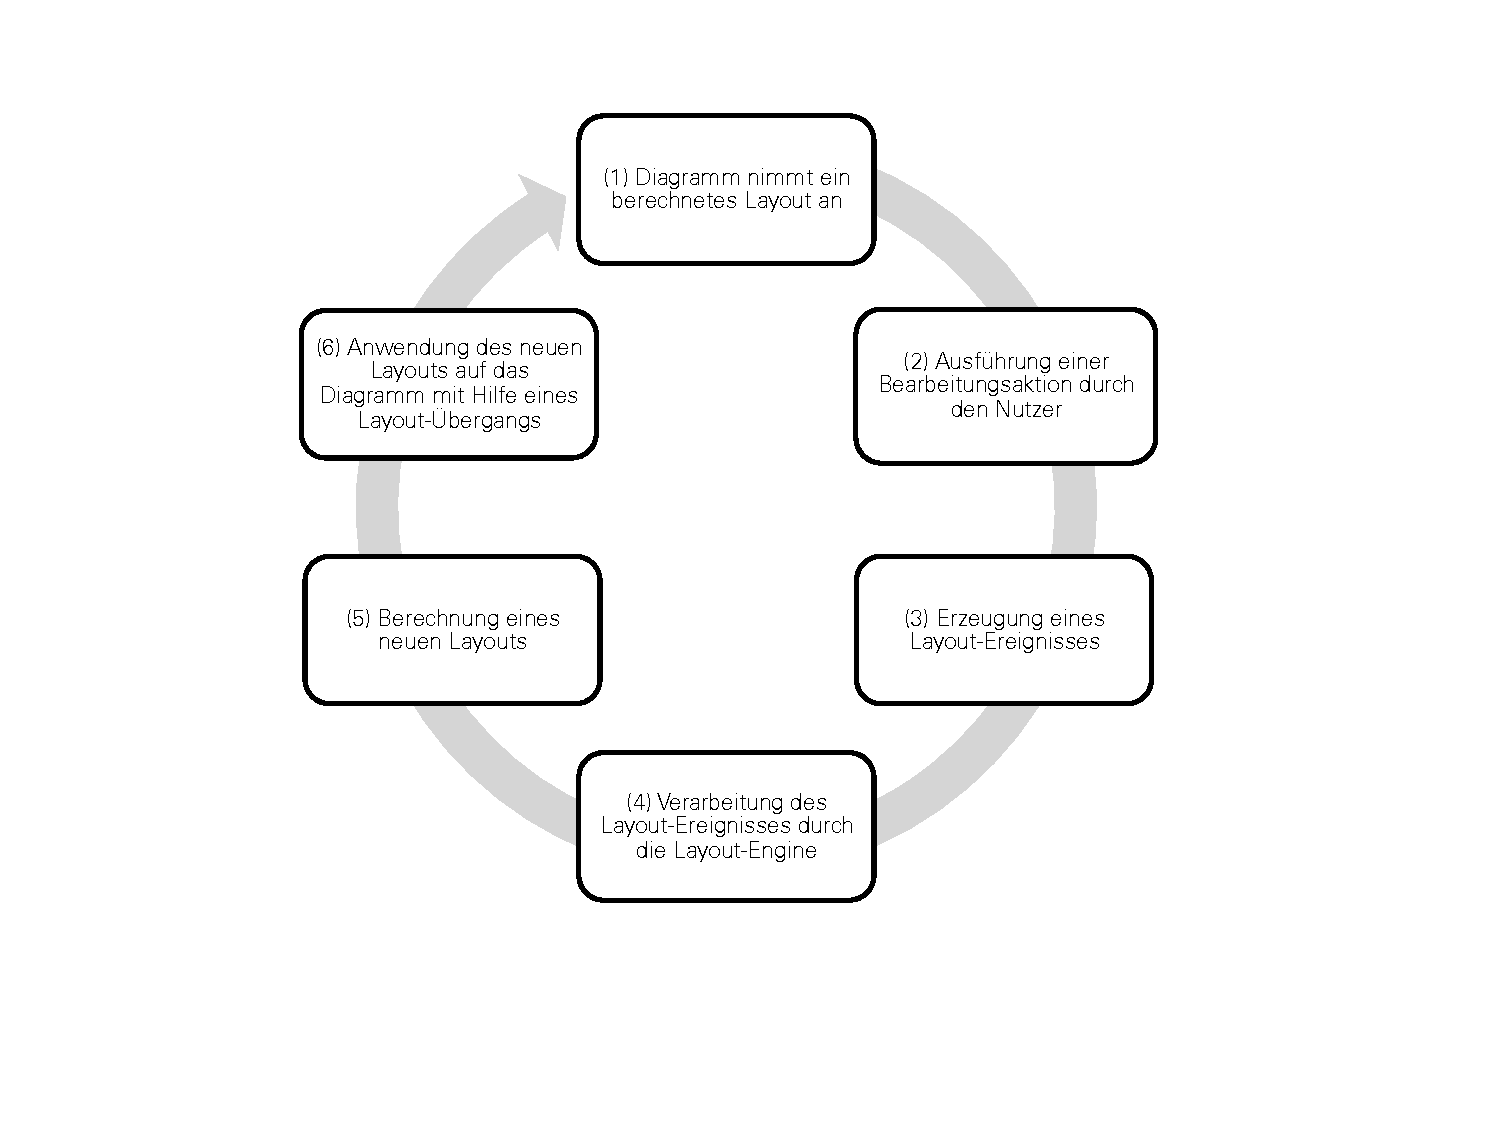
\includegraphics[scale=0.75]{assets/interaction-loop}
    \caption{Die Interaktionsschleife des präsentierten Ansatzes}
    \label{fig:interaction-loop}
\end{figure}

Den Kern des Ansatzes bildet eine Interaktionsschleife, die sich aus mehreren Schritten zusammensetzt und in Abbildung \ref{fig:interaction-loop} illustriert ist. Zunächst befindet sich das bearbeitete Diagramm in einem stabilen Zustand und nimmt ein berechnetes Layout an (Schritt 1). Der Nutzer kann die Interaktion auslösen, indem er eine \textbf{Bearbeitungsaktion} ausführt, die mit Hilfe von \textbf{Bedienungsmechanismen} im Diagramm realisiert und veranschaulicht wird (Schritt 2). Für jede Bearbeitungsaktion werden ein oder mehrere \textbf{Layout-Ereignisse} erzeugt, die die bewirkte Änderung im Diagramm beschreiben (Schritt 3). Diese Layout-Ereignisse werden durch eine \textbf{Layout-Engine} verarbeitet, die für den Typ des Diagramms speziell angepasst ist (Schritt 4). Die Layout-Engine verwaltet intern Instanzen von \textbf{Layout-Patterns}, die die Struktur des Diagramms beschreiben. Neben der instanziierten Layout-Patterns bilden auch der aktuelle Inhalt und das Layout des Diagramms die Grundlage für die Layout-Berechnung. Diese wird im nächsten Schritt durchgeführt (Schritt 5). Anschließend wird das neu berechnete Layout auf das Diagramm angewendet und mit Hilfe eines \textbf{Layout-Übergangs} visualisiert (Schritt 6). Durch die Wiederholung dieser Schritte entsteht der gesamte Bearbeitungsprozess. Die einzelnen genannten Bestandteile und Phasen der Layout-Berechnung werden in weiteren Abschnitten im Detail erläutert.

\section{Mechanismen der Interaktion}
\label{sec:interaction-mechanisms}

Das Kriterium \ref{req:editing-support} erfordert eine Möglichkeit der Bearbeitung des Diagramms. Der Nutzer soll in der Lage sein, neue Knoten und Kanten hinzuzufügen und bestehende Knoten und Kanten zu manipulieren bzw. zu löschen. Durch das Kriterium \ref{req:interactivity} wird gefordert, dass die Bearbeitung interaktiv erfolgt. Dies wird durch die Unterstützung von \textbf{Bearbeitungsaktionen} gewährleistet, die die Grundlage der Interaktion bilden. Die Bearbeitungsaktionen werden in Abschnitt \ref{subsec:edit-actions} im Detail beschrieben.

Weiterhin sollen die Möglichkeiten der Interaktion eingeschränkt werden, um das Ablenken durch die eventuellen Layout-Anpassungen zu minimieren (Kriterium \ref{req:focus-on-the-content}). Dies wird durch die Einschränkung der aus den manuellen Layout-Ansätzen (siehe Abschnitt \ref{sec:manual-layout}) bekannten freien Positionierung der Knoten und den Einsatz eines \textbf{neuen Bedienungsmechanismus} für die Verschiebungsaktion erreicht, dem sich der Abschnitt \ref{subsec:temporary-layer-mechanism} widmet.

Die Erhaltung des mentalen Modells (Kriterium \ref{req:mental-map}) wird durch eine \textbf{Animation der Layout-Übergänge} gewährleistet. Dies wird in Abschnitt \ref{subsec:layout-transitions} thematisiert.

\subsection{Bearbeitungsaktionen}
\label{subsec:edit-actions}

Die interaktiven Ansätze werden in Editoren eingesetzt, die in der Regel über einen Canvas verfügen. Der Canvas ist ein rechteckiger Bereich des Editor-Fensters, in dem das Diagramm dargestellt wird und in dem die Interaktion mit dem Diagramm stattfindet. Die Interaktion setzt sich aus Bearbeitungsaktionen zusammen, die durch den Nutzer ausgeführt werden. Um das Kriterium \ref{req:gui} zu erfüllen, sollen alle Bearbeitungsaktionen auf GUI-Techniken basieren.

In dieser Arbeit werden die grundlegenden Bearbeitungsaktionen präsentiert, die insbesondere für die Entwicklung des Prototyps (siehe Kapitel \ref{chapter:prototype}) eine wichtige Rolle spielen. Natürlich ist eine Erweiterung der unterstützten Bearbeitungsaktionen möglich.

Je nach der Art der Modifizierung lassen sich die Bearbeitungsaktionen in zwei Gruppen unterteilen. Zum einen sind das Aktionen, die den Inhalt des Diagramms modifizieren und zum anderen sind das Aktionen, die das Layout des Diagramms modifizieren, ohne den Inhalt zu verändern.

\subsubsection{Bearbeitungsaktionen zur Modifizierung des Inhalts}

Zu den Bearbeitungsaktionen, die den Inhalt verändern, gehört das Hinzufügen und Löschen von Knoten bzw. Kanten und die Veränderung ihrer Eigenschaften wie z.B. das Umbenennen der Knoten. Da die Intention für die Ausführung dieser Aktionen nicht die Anpassung des Layouts ist, weisen diese Aktionen ein verzögertes Feedback auf, d.h. das Layout wird erst nach der Beendigung der Bearbeitung angepasst\footnote{Eine Ausnahme bildet das Hinzufügen eines neuen Knoten, das sich ähnlich wie die Verschiebungsaktion aus Abschnitt \ref{subsubsec:edit-action-for-modifying-layout} verhält.}.

\subsubsection{Bearbeitungsaktionen zur Modifizierung des Layouts}
\label{subsubsec:edit-action-for-modifying-layout}

Der einzige Vertreter der Bearbeitungsaktionen, die ausschließlich das Layout modifizieren, ist die Verschiebung eines Knotens. Aufgrund der Einschränkung der freien Positionierung wird durch die Verschiebung eine Empfehlung für die Position eines Knotens angegeben. Diese Aktion macht sich einen neuen Bedienungsmechanismus zunutze, der ein unmittelbares Feedback aufweist und näher in Abschnitt \ref{subsec:temporary-layer-mechanism} beschrieben wird. Dieser Mechanismus bildet die Grundlage des gesamten Ansatzes.

\subsection{Mechanismus der temporären Schicht}
\label{subsec:temporary-layer-mechanism}

Alle interaktiven Ansätze für das Layout von Diagrammen aus dem Kapitel \ref{chapter:existing-approaches} bis auf das \enquote{Smart Layout} in \textit{MindNode} (siehe Abschnitt \ref{subsubsec:smart-layout-in-mindnode}) unterstützen \textbf{freie Positionierung} der Objekte im Diagramm. Diese Art der Bedienung wird im manuellen Layout zusätzlich um temporäre Hilfefunktionen (siehe Abschnitt \ref{sec:manual-layout}) und in Struktur-basierten benutzergesteuerten Ansätzen um Möglichkeit der Erzeugung von Strukturregeln (siehe Abschnitt \ref{subsec:structure-based-user-controlled-approaches}) erweitert. Durch diese Erweiterungen wird die freie Positionierung eingeschränkt, wodurch in der Regel ein besseres Layout des Diagramms erreicht werden kann. Dahingegen ist die freie Positionierung in \enquote{Smart Layout} in \textit{MindNode} und dem in dieser Arbeit präsentierten Ansatz \textbf{nicht gestattet}. Stattdessen wird durch die Verschiebung der Objekte ihre ungefähre Position angegeben, die intern ausgewertet wird und eine Anpassung des Layouts bewirkt.

Dieses Verhalten wird für die Verschiebungsaktion der Knoten eingesetzt, indem bei der Verschiebung eines Knotens eine temporäre Schicht erzeugt wird, in der sich der Knoten frei positionieren lässt. Im Diagramm wird der manipulierte Knoten durch einen Platzhalter repräsentiert, der nur zulässige Positionen annehmen kann. Dieser Mechanismus basiert auf der Technik \textbf{\enquote{Drag and Drop}} und ist in drei Phasen aufgeteilt. Im Folgendem wird er an einem Beispiel detailliert erklärt.

Bevor die Verschiebungsaktion beginnen kann, müssen sich im Canvas einige Knoten befinden, so wie es der Fall in Abbildung \ref{fig:movement-action-example-a} ist.

In der ersten Phase wird ein Knoten im Canvas angeklickt, was in Abbildung \ref{fig:movement-action-example-b} durch einen Mauszeiger gekennzeichnet ist. Dabei wird der angeklickte Knoten in eine neu eingefügte \textbf{temporäre Schicht} ausgelagert, die vor dem Canvas positioniert ist, so wie es in Abbildung \ref{fig:temporary-layer-visualization} skizziert ist. Im Canvas wird die ursprüngliche Darstellung des verschobenen Knotens durch einen \textbf{temporären Platzhalter} ersetzt, welcher dem Nutzer die Zielposition des Knotens andeutet. Der Platzhalter ist in Abbildungen \ref{fig:movement-action-example-c} und \ref{fig:temporary-layer-visualization} durch ein Rechteck repräsentiert, das mit einer grauen gestrichelten Linie umrandet ist.

\vspace{0.5cm}

\begin{figure}[hbt]
    \newcommand{\subfigurewidth}{0.28\textwidth}
    \newcommand{\graphicsscale}{1.2}
    \centering
    \begin{subfigure}{\subfigurewidth}
        \centering
        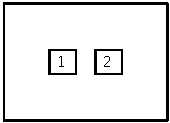
\includegraphics[scale=\graphicsscale]{assets/movement-action-example-a}
        \caption{}
        \label{fig:movement-action-example-a}
    \end{subfigure}
    \begin{subfigure}{\subfigurewidth}
        \centering
        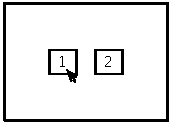
\includegraphics[scale=\graphicsscale]{assets/movement-action-example-b}
        \caption{}
        \label{fig:movement-action-example-b}
    \end{subfigure}
    \begin{subfigure}{\subfigurewidth}
        \centering
        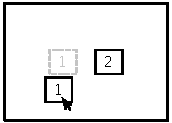
\includegraphics[scale=\graphicsscale]{assets/movement-action-example-c}
        \caption{}
        \label{fig:movement-action-example-c}
    \end{subfigure}
    \begin{subfigure}{\subfigurewidth}
        \centering
        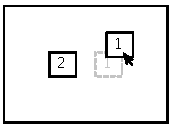
\includegraphics[scale=\graphicsscale]{assets/movement-action-example-d}
        \caption{}
        \label{fig:movement-action-example-d}
    \end{subfigure}
    \begin{subfigure}{\subfigurewidth}
        \centering
        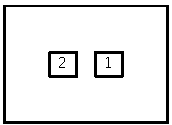
\includegraphics[scale=\graphicsscale]{assets/movement-action-example-e}
        \caption{}
        \label{fig:movement-action-example-e}
    \end{subfigure}
    \caption{Beispiel einer Verschiebungsaktion}
    \label{fig:movement-action-example}
\end{figure}

\begin{figure}[hbt]
    \newcommand{\subfigurewidth}{0.35\textwidth}
    \newcommand{\graphicsscale}{0.95}
    \centering
    \begin{subfigure}{\subfigurewidth}
        \centering
        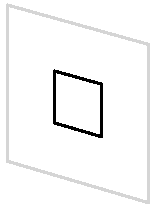
\includegraphics[scale=\graphicsscale]{assets/temporary-layer-visualization-a}
        \caption{}
    \end{subfigure}
    \begin{subfigure}{\subfigurewidth}
        \centering
        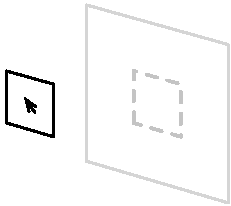
\includegraphics[scale=\graphicsscale]{assets/temporary-layer-visualization-b}
        \caption{}
    \end{subfigure}
    \caption{Darstellung der temporären Schicht vor dem Canvas}
    \label{fig:temporary-layer-visualization}
\end{figure}

In der zweiten Phase findet eine Bewegung des Mauszeigers statt. Da die temporäre Schicht an den Mauszeiger gebunden ist, wird die ausgelagerte Darstellung des Knotens frei mit dem Mauszeiger bewegt, währenddessen der Platzhalter im Canvas seine Position zunächst nicht ändert. Dies ist in Abbildung \ref{fig:movement-action-example-c} illustriert.

Die Position des Mauszeigers wird nach jeder Bewegung ausgewertet und sobald sich der Mauszeiger in einem bestimmten Bereich des Diagramms befindet, für den das Layout geändert werden soll, wird das Layout im unterliegenden Canvas mit Hilfe einer Animation (siehe Abschnitt \ref{subsec:layout-transitions}) angepasst. Dabei wird die Änderung der Layout-Eigenschaften des verschobenen Knotens auf den Platzhalter angewendet, so wie es in Abbildung \ref{fig:movement-action-example-d} dargestellt ist. Durch die Anpassung des Layouts während der Interaktion wird ein unmittelbares Feedback erreicht (Kriterium \ref{req:immediate-feedback}). Dagegen wird das Layout in \textit{MindNode} (siehe Abschnitt \ref{subsubsec:smart-layout-in-mindnode}) erst nach dem Loslassen der Maustaste angepasst und damit das Feedback verzögert.

Dieser Abschnitt beschäftigt sich ausschließlich mit der Beschreibung der Interaktion, die konkrete Funktionsweise der Layout-Berechnung kann in Abschnitt \ref{sec:layout-calculation} nachgelesen werden.

Die dritte Phase beginnt mit dem Loslassen der Maustaste. Danach springt der verschobene Knoten auf seine Zielposition hin, nämlich die Position des Platzhalters. Anschließend werden der Platzhalter sowie die temporäre Schicht entfernt und die Verschiebungsaktion wird beendet. Die Abbildung \ref{fig:movement-action-example-e} zeigt den Endzustand.

\subsection{Layout-Übergänge}
\label{subsec:layout-transitions}

In vorhergehenden Abschnitten wurde beschrieben, dass nach der Änderung des Inhalts bzw. während der Verschiebung eines Knotens das Layout angepasst wird. Konkret handelt es sich um einen Übergang vom aktuellen zu einem neu berechneten Layout. Um diese Übergänge für den Nutzer nachvollziehbar zu machen, wird eine Animation eingesetzt, die insbesondere für die Erhaltung des mentalen Modells sorgt (Kriterium \ref{req:mental-map}).

\section{Layout-Patterns}
\label{sec:layout-patterns}

Die Layout-Patterns dienen der Beschreibung der Struktur des Layouts eines Diagramms. Ähnlich wie in \cite{Maier12A-Pattern-based} handelt es sich um allgemeine wiederverwendbare Lösungen für Layout-Probleme. Die Auffassung der Layout-Patterns in dieser Arbeit ist im Vergleich zu dem Konzept aus \cite{Maier12A-Pattern-based} (siehe Abschnitt \ref{subsubsec:pattern-based-approach}) sehr vereinfacht. Zum einen werden die Layout-Patterns nicht an einem separaten Metamodell definiert, sondern direkt auf dem Metamodell der konkreten Syntax des gewählten Beispiels. Zum anderen besitzen die Layout-Patterns keine komplexe Struktur der Regelausführung wie in \cite{Maier12A-Pattern-based}.

Die präsentierten Layout-Patterns wurden von den in Abschnitt \ref{sec:aesthetics-criteria} aufgeführten ästhetischen Kriterien abgeleitet und orientieren sich insbesondere an der Unterstützung der Interaktion u.a. durch das Konzept der Variierung. Des Weiteren führt diese Arbeit eine Aufteilung auf implizite und explizite Patterns ein. Die Problematik der Layout-Patterns wird im Folgenden detailiert behandelt.

\subsection{Implizite Layout-Patterns}
\label{subsec:implicit-layout-patterns}

Die impliziten Layout-Patterns beschreiben allgemeine Eigenschaften für die Layout-Be\-rech\-nung. Dafür werden keine expliziten Strukturregeln erzeugt, wie das der Fall bei den expliziten Layout-Patterns (siehe Abschnitt \ref{subsec:explicit-layout-patterns}) ist, sondern sie werden von dem Algorithmus der Layout-Berechnung als geltend angenommen.

\subsubsection{Größe der Knoten}

In allen interaktiven Ansätzen für das Layout von Diagrammen aus dem Kapitel \ref{chapter:existing-approaches} hat der Nutzer die Möglichkeit die Größe der Objekte zu verändern. Weiterhin werden in dem allgemeinen Ansatz aus \cite{Maier12A-Pattern-based} Layout-Patterns präsentiert, die Regeln für die Größe der Objekte beschreiben. Somit ist die Größe der Objekte eine Eigenschaft, die zum einen von dem Nutzer und zu anderem von dem Layout-Algorithmus geändert werden kann.

Dagegen ist die Größe der Knoten in dieser Arbeit ausschließlich durch den Inhalt des Knotens bestimmt. Sie nimmt zunächst eine minimale Größe an und wenn der Inhalt\footnote{Für eine Klasse der Notationssprache UML handelt es sich um ihre Bezeichnung und die Liste der Attribute und Methoden.} in den Knoten mit der minimalen Größe nicht passt, wird der Knoten entsprechend erweitert. Somit kann die Größe der Knoten weder durch den Nutzer noch durch die Layout-Berechnung geändert werden. Dieses implizite Layout-Pattern fördert insbesondere die Konzentration auf den Inhalt (Kriterium \ref{req:focus-on-the-content}) und die ästhetische Gestaltung (Kriterium \ref{req:aesthetics-criteria}).

\subsubsection{Verhinderung der Knoten-Überlappung}
\label{subsubsec:prevention-of-node-overlap}

Dadurch dass die Größe der Knoten bekannt ist und die Position der Knoten berechnet wird, kann die Knoten-Überlappung verhindert werden. Dies trägt der Ästhetik des Diagramms (Kriterium \ref{req:aesthetics-criteria}) und insbesondere der Einhaltung der Abstände zwischen den Knoten (Prinzip \ref{pri:distances}) bei.

\subsubsection{Zentrierung des Diagramm-Inhalts}
\label{subsubsec:centering-of-diagram-content}

Die Zentrierung des Diagramm-Inhalts ist ein weiteres ästhetisches Layout-Pattern, das eine eindeutige Bestimmung des Layouts ermöglicht. Die Berechnung des Layouts erfolgt relativ und wird dermaßen auf das Diagramm angewendet, so dass der Diagramm-Inhalt immer in die Mitte des Canvas platziert wird und dadurch die Zeichenfläche optimal ausgenutzt wird (Prinzip \ref{pri:drawing-area}). Dies wird in Abbildung \ref{fig:layout-pattern-centered-content} veranschaulicht.

\begin{figure}[hbt]
    \centering
    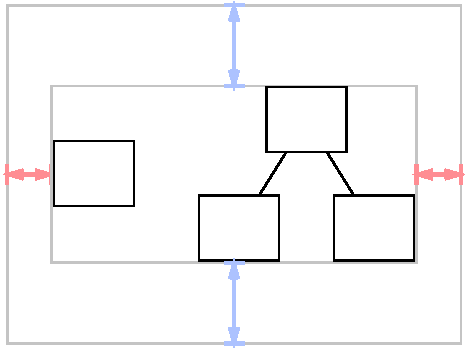
\includegraphics{assets/layout-pattern-centered-content}
    \caption{Die Zentrierung des Diagramm-Inhalts im Canvas}
    \label{fig:layout-pattern-centered-content}
\end{figure}

Neben der Förderung der Ästhetik (Kriterium \ref{req:aesthetics-criteria}) wird vor allem die Einschränkung der freien Positionierung (siehe Abschnitt \ref{subsec:temporary-layer-mechanism}) möglich gemacht.

\subsection{Explizite Layout-Patterns}
\label{subsec:explicit-layout-patterns}

Die expliziten Layout-Patterns referenzieren Knoten im Diagramm und beschreiben deren Struktur anhand von geometrischen Eigenschaften. Während der Erstellung eines Diagramms werden ähnlich wie in \cite{Maier12A-Pattern-based} \textbf{Instanzen der Layout-Patterns} verwaltet. Im Gegensatz zu \cite{Maier12A-Pattern-based} erfolgt die Verwaltung automatisch und basiert auf dem Inhalt des Diagramms. Der Nutzer hat daher keine Möglichkeit die Layout-Patterns selbst zu erstellen\footnote{Eine eventuelle Möglichkeit der Erstellung von Layout-Patterns durch den Nutzer wird in Abschnitt \ref{sec:outlook} diskutiert.}.

Um eine Art der Manipulation der Knoten zu ermöglichen, wird das Konzept der \textbf{Variierung der expliziten Layout-Patterns} eingeführt. Je nach der Art des expliziten Layout-Patterns kann der Nutzer zwischen mehreren Variationen der Anordnung der Knoten (z.B. Reihenfolge) wählen. Das endgültige Layout wird jedoch durch die Geometrie bestimmt. Diese Art der Manipulation fördert die Konzentration auf den Inhalt und ergänzt die Einschränkung der freien Positionierung (Kriterium \ref{req:focus-on-the-content}).

Im Folgenden werden zwei konkrete explizite Layout-Patterns vorgestellt, nämlich das Ausrichtungspattern (siehe Abschnitt \ref{subsubsec:alignment-pattern}) und das T-Shape-Pattern (siehe Abschnitt \ref{subsubsec:t-shape-pattern}). Mit der Implementierung der expliziten Layout-Patterns im Prototyp beschäftigt sich der Abschnitt \ref{subsubsec:patterns}.

\subsubsection{Ausrichtungspattern}
\label{subsubsec:alignment-pattern}

Das Ausrichtungspattern beschreibt eine Reihe an Knoten und kombiniert die Ausrichtung und Verteilung der Knoten aus dem manuellen Layout (siehe Abschnitt \ref{subsubsec:alignment-and-distribution}) bzw. die Layout-Patterns zum Ausrichten und Verteilen aus \cite[S.143ff und S.136ff]{Maier12A-Pattern-based}. Die Knoten werden in einer horizontalen oder vertikalen Reihe gleichmäßig verteilt und an die Kanten bzw. Mittelpunkte ausgerichtet. In den Abbildungen \ref{fig:layout-pattern-alignment-center} und \ref{fig:layout-pattern-alignment-top} werden zwei Beispiele für das horizontale Verteilen mit der Ausrichtung an die oberen Kanten bzw. Mittelpunkte gezeigt. Die gleichen Abstände sind mit roten Pfeilen und die Anordnung durch eine graue Linie gekennzeichnet.

\begin{figure}[hbt]
    \centering
    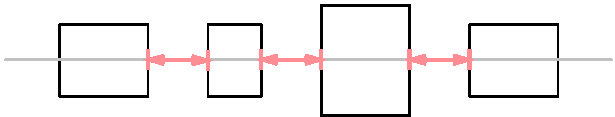
\includegraphics{assets/layout-pattern-alignment-center}
    \caption{Horizontales Ausrichtungspattern mit der Ausrichtung an die Mittelpunkte}
    \label{fig:layout-pattern-alignment-center}
\end{figure}

\begin{figure}[hbt]
    \centering
    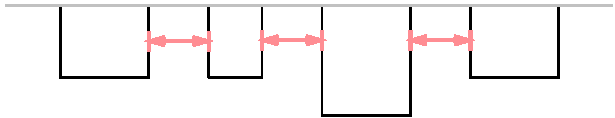
\includegraphics{assets/layout-pattern-alignment-top}
    \caption{Horizontales Ausrichtungspattern mit der Ausrichtung an die oberen Kanten}
    \label{fig:layout-pattern-alignment-top}
\end{figure}

Die Variierung des Ausrichtungspatterns besteht in der Veränderung der Reihenfolge der ausgerichteten Knoten. Somit hat ein Ausrichtungspattern mit drei Knoten sechs möglichen Variationen. Dies ist in Abbildung \ref{fig:layout-pattern-alignment-variations} veranschaulicht.

\vspace{0.5cm}

\begin{figure}[hbt]
    \centering
    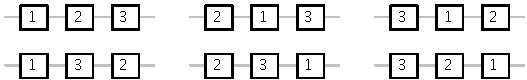
\includegraphics[scale=1.3]{assets/layout-pattern-alignment-variations}
    \caption{Mögliche Variationen des Ausrichtungspatterns mit drei Knoten}
    \label{fig:layout-pattern-alignment-variations}
\end{figure}

\subsubsection{T-Shape-Pattern}
\label{subsubsec:t-shape-pattern}

Das T-Shape-Pattern beschreibt die Struktur von Knoten, die in der Form des Buchstabes \enquote{T} angeordnet sind. Dies ist insbesondere für die Darstellung von Hierarchien in Diagrammen von Bedeutung (Prinzip \ref{pri:hierarchies}).

Ein Knoten hat eine spezielle Rolle und ist den anderen Knoten übergeordnet. Die untergeordneten Knoten sind ähnlich wie in dem Ausrichtungspattern gleichmäßig in einer Reihe angeordnet und an die Kanten ausgerichtet, die sich am nächsten zu dem übergeordneten Knoten befinden. Der übergeordnete Knoten befindet sich in einem definierten Abstand zu den untergeordneten Knoten und ist mittig ausgerichtet. In Abbildung \ref{fig:layout-pattern-t-shape} ist ein Beispiel des T-Shape-Patterns dargestellt, in dem der übergeordnete Knoten oben positioniert ist. Die Abstände sind mit farbigen Pfeilen und die Ausrichtung mit grauen Linien gekennzeichnet. Natürlich gibt es weitere Formen des T-Shape-Patterns, in den sich der übergeordnete Knoten links, unten oder rechts befindet.

\begin{figure}[hbt]
    \centering
    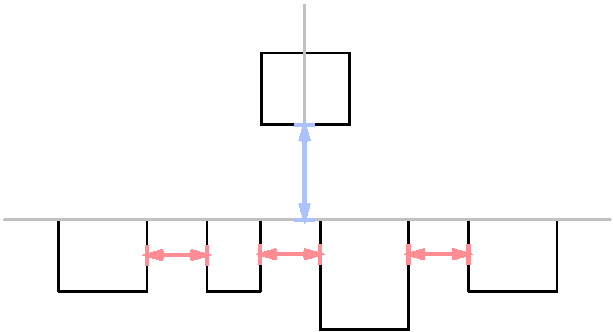
\includegraphics{assets/layout-pattern-t-shape}
    \caption{Das T-Shape-Pattern mit dem oben positionierten übergeordneten Knoten}
    \label{fig:layout-pattern-t-shape}
\end{figure}

Durch das T-Shape-Pattern wird das Ausrichtungspattern erweitert, indem die Reihe der untergeordneten Knoten um einen übergeordneten Knoten ergänzt wird. Identisch wie bei dem Ausrichtungspattern lässt sich bei dem T-Shape-Pattern die Reihenfolge der untergeordneten Knoten verändern.

\section{Berechnung des Layouts}
\label{sec:layout-calculation}

Wie bereits in Abschnitt \ref{subsec:edit-actions} erläutert wurde, werden während der Bearbeitung eines Diagramms Aktionen durch den Nutzer ausgeführt. Für die ausgeführten Bearbeitungsaktionen werden \textbf{Layout-Ereignisse} generiert, die eine Beschreibung der manipulierten bzw. geänderten Knoten und Kanten sowie die Parameter der Interaktion wie z.B. die Position des Mauszeigers beinhalten. Die \textbf{Layout-Engine}, die für die Berechnung des Layouts zuständig ist, nimmt die erzeugten Layout-Ereignisse entgegen, verarbeitet sie und passt das Layout des Diagramms an. Mit der Layout-Engine beschäftigt sich näher der Abschnitt \ref{subsec:layout-engine}. Der Prozess der Verarbeitung der Layout-Ereignisse wird in Abschnitt \ref{subsec:processing-of-layout-events} beschrieben. Schließlich werden die konkreten Layout-Algorithmen in Abschnitt \ref{subsec:concrete-layout-algorithms} vorgestellt.

\subsection{Layout-Engine}
\label{subsec:layout-engine}

Die Layout-Engine ist ein zentraler Bestandteil des präsentierten Ansatzes. Sie ist mit dem bearbeiteten Diagramm verknüpft, dessen Layout sie berechnet. Des Weiteren verwaltet sie Instanzen von expliziten Layout-Patterns (siehe Abschnitt \ref{subsec:explicit-layout-patterns}), wodurch die Struktur des Diagramms beschrieben wird.

Damit der Prozess der Verarbeitung von Layout-Ereignissen beginnen kann, muss sich die Layout-Engine in einem \textbf{validen Zustand} befinden. Dies wird entweder durch das Speichern des Zustandes der Layout-Engine oder durch die Berechnung eines initialen Layouts gewährleistet. Die Aufgabe der zuletzt genannten Option besteht darin, die expliziten Layout-Patterns ähnlich wie in \cite{MaierMinas13A-Pattern-based} anhand des Inhalts des Diagramms automatisiert zu instanziieren.

\subsection{Verarbeitung der Layout-Ereignisse}
\label{subsec:processing-of-layout-events}

Der Lebenszyklus der Layout-Engine besteht aus der sequenziellen Verarbeitung der Layout-Ereignisse, die nach bzw. während der Ausführung von Bearbeitungsaktionen erzeugt werden. Sobald die Layout-Engine ein Layout-Ereignis empfängt, verarbeitet sie dieses sofort. Der Prozess der Verarbeitung der Layout-Ereignisse besteht aus zwei Phasen und ist in Abbildung \ref{fig:processing-of-layout-events} schematisiert.

\begin{figure}[hbt]
    \centering
    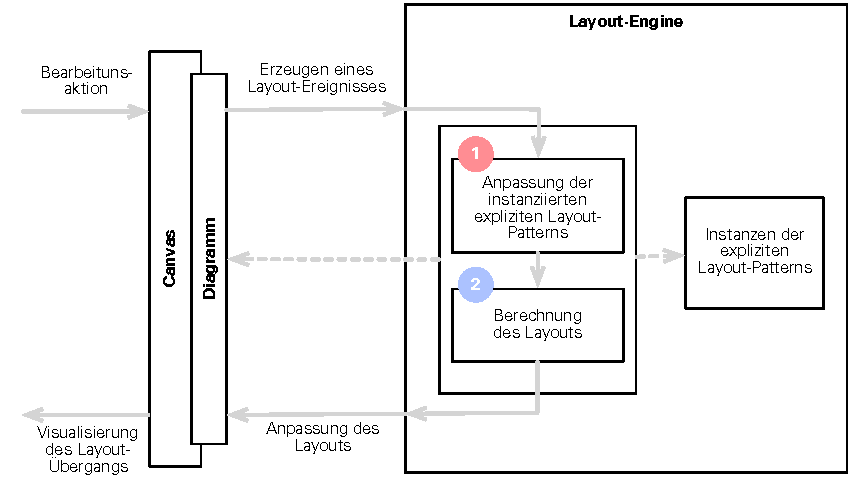
\includegraphics[width=\textwidth]{assets/processing-of-layout-events}
    \caption{Schema der Verarbeitung der Layout-Ereignisse}
    \label{fig:processing-of-layout-events}
\end{figure}

Je nach der Art des Layout-Ereignisses werden in der \textbf{ersten Phase} die Instanzen der expliziten Layout-Patterns angepasst, indem:

\begin{itemize}
    \item neue Layout-Patterns erstellt bzw. bestehende  Layout-Patterns gelöscht,
    \item die Referenzen auf Knoten der bestehenden Layout-Patterns modifiziert
    \item oder die bestehenden Layout-Patterns variiert werden.
\end{itemize}

Insbesondere wird dabei von dem aktuellen Zustand des Diagramms, den bereits instanziierten Layout-Patterns und der Information über die Interaktion Gebrauch gemacht. Das genaue Verhalten der Anpassung der Layout-Patterns ist jedoch von einer konkreten Layout-Engine abhängig, die für den gewählten Diagrammtyp ausgelegt ist. Dieser Sachverhalt wird in Abschnitt \ref{subsec:concrete-layout-algorithms} diskutiert und an konkreten Beispielen illustriert.

In der \textbf{zweiten Phase} wird das \textbf{Layout} berechnet, welches durch die impliziten und instanziierten expliziten Layout-Patterns eindeutig bestimmt ist und die Positionen für alle Knoten im Diagramm enthält\footnote{Es wäre möglich, auch weitere Layout-Eigenschaften wie Routen für die Kanten oder Parameter der Layout-Übergänge zu berechnen. Dies wurde in dieser Arbeit aus zeitlichen Gründen jedoch außer Acht gelassen.}. Sofern sich das neu berechnete Layout von dem aktuellen unterscheidet, wird das neue Layout auf das Diagramm angewendet und dadurch ein Layout-Übergang erzeugt (siehe Abschnitt \ref{subsec:layout-transitions}). Damit wird die Verarbeitung des Layout-Ereignisses abgeschlossen und der gesamte Vorgang fängt für das nächste Layout-Ereignis von vorne an.

Im Rahmen der Konzeption und Entwicklung wurde zunächst ein Algorithmus entworfen, der für die Verschiebung eines Knotens alle erreichbaren Layouts berechnet hat. Des Weiteren wurde der Canvas in Bereiche aufgeteilt. Dabei wurde jeder Bereich auf ein berechnetes Layout abgebildet. Während der Ausführung der Verschiebungsaktion wurde ein Layout-Übergang genau dann ausgelöst, wenn der Mauszeiger in einen anderen Bereich bewegt wurde. Da die Aufteilung der Bereiche nach jedem Layout-Übergang nicht aktualisiert wurde, war sie oft nach dem ersten Layout-Übergang ungültig. Später wurde festgelegt, dass dieser Algorithmus nicht hinreichend ist.

In dem präsentierten Ansatz wird für die Verschiebungsaktion ein Layout-Ereignis für jede Bewegung des Mauszeigers generiert und verarbeitet. Dabei sollen bei dem Entwurf eines konkreten Algorithmus folgende Eigenschaften beachtet werden:

\newpage

\begin{itemize}

\item
\textbf{Stabilität}
Während der Ausführung der Verschiebungsaktion soll ein Layout-Übergang erst nach einer deutlichen Bewegung des Mauszeigers durch den Nutzer ausgelöst werden.

\item
\textbf{Erreichbarkeit des Ausgangslayouts}
Das Layout, das ein Diagramm annimmt, wenn die Verschiebungsaktion beginnt, soll im Verlauf der Ausführung der Verschiebungsaktion stets erreichbar sein.

\end{itemize}

\subsection{Konkrete Layout-Algorithmen}
\label{subsec:concrete-layout-algorithms}

In Abschnitt \ref{subsec:processing-of-layout-events} wurde der Rumpf des Algorithmus für die Berechnung des Layouts vorgestellt. Dabei wurde nicht auf die interne Funktionsweise der Layout-Engine eingegangen. Das liegt daran, dass die Layout-Engine ein unterschiedliches Verhalten für verschiedene \textbf{Diagrammtypen} aufweisen soll, denn jeder Diagrammtyp (z.B. Klassendiagramm, Zustandsdiagramm, Flowchart usw.) hat aufgrund der Syntax- und Semantikregeln spezielle Anforderungen an das ästhetische Layout. Nur dadurch kann das Kriterium \ref{req:syntax-and-semantics} erfüllt werden.

Die in dieser Arbeit präsentierten Algorithmen basieren auf der visuellen Sprache der Klassendiagramme der Notationssprache UML. Allerdings handelt es sich um keine vollständigen Algorithmen für das Layout von Klassendiagrammen, sondern um zwei relativ einfache Algorithmen, deren Aufgabe es ist, die eingeführten Mechanismen der Interaktion zu validieren und damit das gesamte Konzept zu prüfen. Daher wird der Einfachheit halber kein UML-Metamodell eingesetzt und die Syntax wird stark eingeschränkt. Es werden nur vereinfachte Klassen (Knoten) und Vererbungsrelationen (Kanten) unterstützt.

\subsubsection{Algorithmus für das horizontale Layout}
\label{subsubsec:horizontal-layout-algorithm}

Der Algorithmus für das horizontale Layout ordnet alle Klassen eines Klassendiagramms in eine horizontale Reihe an und lässt dabei die Vererbungsrelationen außer Acht.

Die Layout-Engine, die diesen Algorithmus umsetzt, enthält intern eine Instanz des Ausrichtungspatterns (siehe Abschnitt \ref{subsubsec:alignment-pattern}), das alle Klassen des Diagramms referenziert. Dieser Algorithmus hat aus der Sicht des Nutzers keine große Bedeutung und dient ausschließlich als Grundlage für den Algorithmus für das baumbasierte Layout, mit dem sich der Abschnitt \ref{subsubsec:tree-layout-algorithm} beschäftigt.

Nichtsdestotrotz macht der Algorithmus die Mechanismen der Interaktion aus Abschnitt \ref{sec:interaction-mechanisms} verständlich. Insbesondere zeigt die Verschiebungsaktion die Möglichkeit der Änderung der Reihenfolge der Klassen im Diagramm. Dies wird durch die Layout-Engine in eine direkte Variierung des Ausrichtungspatterns übersetzt. Die prototypische Implementierung dieses Algorithmus wird in einem Video unter dem Pfad \texttt{Prototype/Videos/Hori\-zon\-tal-\-Lay\-out-\-De\-mo.mov} auf der eingereichten CD veranschaulicht.

\subsubsection{Algorithmus für das baumbasierte Layout}
\label{subsubsec:tree-layout-algorithm}

Der Algorithmus für das baumbasierte Layout ermöglicht die Modellierung von Vererbungshierarchien in einem Klassendiagramm. Dabei hält er sich an die in Abschnitt \ref{sec:aesthetics-criteria} beschriebene ästhetischen Prinzipien. Insbesondere wird das Prinzip der Darstellung von Hierarchien eingehalten (Prinzip \ref{pri:hierarchies}).

Ähnlich wie bei der Umsetzung des Algorithmus für das horizontale Layout (siehe Abschnitt \ref{subsubsec:horizontal-layout-algorithm}) enthält die Layout-Engine, die den Algorithmus für das baumbasierte Layout umsetzt, eine Instanz des horizontalen Ausrichtungspatterns, das jedoch nicht alle Klassen im Diagramm sondern nur die Wurzelklassen der Vererbungshierarchien referenziert. Durch dieses globale Ausrichtungspattern wird die Reihenfolge der Vererbungshierarchien bestimmt. Während der Erstellung von Vererbungsrelationen zwischen Klassen werden T-Shape-Patterns (siehe Abschnitt \ref{subsubsec:t-shape-pattern}) instanziiert, die die Struktur der Vererbungshierarchien beschreiben und durch die Layout-Engine verwaltet werden. In Abbildung \ref{fig:tree-based-layout} wird ein Beispiel eines Diagramms mit gekennzeichneten Layout-Patterns gezeigt. Die blaue Linie stellt das globale Ausrichtungspattern dar und mit den grünen Linien sind die instanziierten T-Shape-Patterns markiert. Die Vererbungshierarchien sind mit grauen gestrichelten Linien umrandet.

\begin{figure}[hbt]
    \centering
    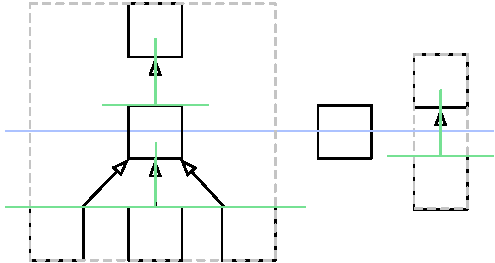
\includegraphics[width=0.7\textwidth]{assets/tree-based-layout}
    \caption{Visualisierung von Instanzen der expliziten Layout-Patterns im baumbasierten Layout}
    \label{fig:tree-based-layout}
\end{figure}

Die Berechnung des endgültigen Layouts erfolgt durch die Zusammensetzung der instanziierten expliziten Layout-Patterns. Dabei wird die oben beschriebene Vereinfachung der Klassendiagramme ausgenutzt und der Algorithmus ist somit ausschließlich für diesen konkreten Fall geeignet. Die Möglichkeit der Entwicklung eines vollständigen Algorithmus für Klassendiagramme wird in Abschnitt \ref{sec:outlook} diskutiert.

Je nachdem welche Klasse verschoben wird, verhält sich die Verschiebungsaktion unterschiedlich. Das Verschieben der Wurzelklassen bewirkt die Änderung der Reihenfolge der Vererbungshierarchien. Im Fall der Verschiebung einer Klasse, die sich in einer Vererbungshierarchie unter der Wurzelklasse befindet, wird die Reihenfolge der Geschwisterklassen angepasst. Dies erfolgt durch die Variierung des zugehörigen T-Shape-Patterns (siehe Abschnitt \ref{subsubsec:t-shape-pattern}). Zum besseren Verständnis der Funktionsweise dieses Algorithmus wird auf ein Video mit der Vorführung der prototypischen Implementierung verwiesen. Das Video ist unter dem Pfad \texttt{Prototype/Videos/Tree-based\--Lay\-out-\-De\-mo.mov} auf der eingereichten CD zu finden.

\section{Abgrenzung zu bestehenden Ansätzen}
\label{sec:current-approaches-comparison}

Im Folgenden wird der oben vorgestellte Ansatz mit bestehenden Ansätzen aus Kapitel \ref{chapter:existing-approaches} verglichen und von ihnen abgegrenzt. Dieser Abschnitt wird nach der in Abschnitt \ref{sec:categorization} präsentierten Kategorisierung in Ansätze für das manuelle (siehe Abschnitt \ref{subsec:comparison-manual-layout}), automatische (siehe Abschnitt \ref{subsec:comparison-automatic-layout}) und interaktive halbautomatische (siehe Abschnitt \ref{subsec:comparison-interactive-layout}) Layout aufgeteilt.

\subsection{Abgrenzung zu den Ansätzen für das manuelle Layout}
\label{subsec:comparison-manual-layout}

Die fundamentale Eigenschaft der Ansätze für das manuelle Layout, die in Abschnitt \ref{sec:manual-layout} vorgestellt wurden, ist die Unterstützung der Freihand-Bearbeitung. Dadurch kann der Nutzer die Layout-Eigenschaften der Objekte im Diagramm wunschgemäß anpassen. Insbesondere schließt dies die freie Positionierung ein. Die Bearbeitung erfolgt interaktiv und die Editoren stellen in der Regel zusätzliche Hilfefunktionen für die Layout-Erstellung zur Verfügung (siehe Abschnitt \ref{subsec:help-functions-for-manual-layout}). Obwohl der präsentierte Ansatz keine Freihand-Bearbeitung unterstützt und speziell die freie Positionierung einschränkt, werden neue Bedienungsmechanismen für die interaktive Bearbeitung des Diagramms eingeführt. Im Vergleich zu den Ansätzen für das manuelle Layout ist der präsentierte Ansatz weniger flexibel, dennoch kann das resultierende Layout durch den Nutzer beeinflusst werden, indem es variiert wird. Diese Einschränkungen in Kombination mit der halbautomatischen Berechnung führen dazu, dass der Aufwand an der Layout-Erstellung wesentlich reduziert wird. Des Weiteren ist es möglich, die syntaktischen und semantischen Regeln der konkreten Diagrammtypen durch den Layout-Algorithmus einzuhalten.

\subsection{Abgrenzung zu den Ansätzen für das automatische Layout}
\label{subsec:comparison-automatic-layout}

Da der präsentierte Ansatz eine direkte Interaktion mit dem Diagramm unterstützt, erfolgt die Eingabe ähnlich wie bei den visuellen Ansätzen für das automatische Layout (siehe Abschnitt \ref{subsec:visual-approaches}) in einer visuellen Sprache. Eine weitere Gemeinsamkeit besteht darin, dass das Layout automatisch berechnet wird. Die Layout-Berechnung wird durch einen Algorithmus durchgeführt, dessen Aufgabe es ist, die Layout-Eigenschaften für die im Diagramm enthaltene Objekte zu bestimmen. Der Layout-Algorithmus in dem präsentierten Ansatz ist zusätzlich für die Verarbeitung der Interaktion ausgelegt (siehe Abschnitt \ref{subsec:processing-of-layout-events}). Dadurch ist der Ansatz im Unterschied zu den Ansätzen für das automatische Layout für interaktive Umgebungen geeignet, denn er ermöglicht eine Anpassung des berechneten Layouts nach den Nutzerpräferenzen. Der Einfluss auf das Layout besteht daher in der Variierung anstatt der Einstellung der Parameter des Layout-Algorithmus, wie das der Fall bei den Ansätzen für das automatische Layout ist. Weiterhin wird durch die Layout-Übergänge das mentale Modell erhalten (siehe Abschnitt \ref{subsec:layout-transitions}). Obwohl der präsentierte Ansatz eine Berechnung des initialen Layouts unterstützt (siehe Abschnitt \ref{subsec:layout-engine}), wird die Möglichkeit der Einbindung in automatisierte Prozesse aufgrund des interaktiven Charakters ausgeschlossen.

Da sich diese Arbeit insbesondere mit den interaktiven Aspekten des Ansatzes beschäftigt, legt sie einen großen Wert auf die Einhaltung der ästhetischen Prinzipien sowohl für Graphen als auch für Klassendiagramme. Im Unterschied zu den speziellen Algorithmen für die Klassendiagramme (siehe Abschnitt \ref{subsec:special-algorithms-for-class-diagrams}) wird deren Unterstützung nur partiell ausgearbeitet und wird der weiteren Forschung überlassen. Diese Problematik wird in Abschnitt \ref{sec:outlook} aufgegriffen.

\subsection{Abgrenzung zu den Ansätzen für das interaktive halbautomatische Layout}
\label{subsec:comparison-interactive-layout}

Der präsentierte Ansatz lässt sich in die Kategorie der Ansätze für das interaktive halbautomatische Layout einordnen (siehe Abschnitt \ref{sec:interactive-semi-automatic-layout}) und besitzt somit viele Gemeinsamkeiten mit Ansätzen aus dieser Kategorie. Die Eigenschaft, die diese Ansätze ausmacht, ist die Unterstützung der interaktiven Bearbeitung des Diagramms. Jedoch kann das Diagramm in dem präsentierten Ansatz durch den Nutzer nicht frei bearbeitet werden. Insbesondere wird die Anpassung der Layout-Eigenschaften nicht gestattet. Dagegen werden neue Mechanismen der Interaktion eingeführt (siehe Abschnitt \ref{sec:interaction-mechanisms}), die die Bearbeitungsmöglichkeiten einschränken und die Konzentration auf den Inhalt fördern.

In \cite[S.5]{Maier12A-Pattern-based} wird aufgeführt, dass die Einhaltung der ästhetischen Prinzipien im dynamischen Kontext eine geringere Rolle als die Erhaltung des mentalen Modells spielt. Der präsentierte Ansatz strebt an, diese These durch eine gleichzeitige Unterstützung beider Kriterien zu widerlegen. Die ästhetischen Prinzipien werden durch die automatische Layout-Berechnung berücksichtigt und da die Interaktion auf die Variierung des berechneten Layouts beschränkt ist, können sie durch den Nutzer nicht verletzt werden. Des Weiteren sorgen die Layout-Übergänge (siehe Abschnitt \ref{subsec:layout-transitions}) für die Erhaltung des mentalen Modells.

Ähnlich wie in den Struktur-basierten benutzergesteuerten Ansätzen (siehe Abschnitt \ref{subsec:structure-based-user-controlled-approaches}), wird in dem präsentierten Ansatz das Layout mit Hilfe von Strukturregeln beschrieben, die einen persistenten Charakter haben. Obwohl der Begriff der Layout-Patterns von \cite{Maier12A-Pattern-based} übernommen wurde, unterscheiden sich die Konzepte stark voneinander. Die konkreten Unterschiede werden in Abschnitt \ref{sec:layout-patterns} sowie \ref{subsec:explicit-layout-patterns} diskutiert.

\section{Zusammenfassung}
\label{sec:approach-summary}

In diesem Kapitel wurde das Konzept eines neuartigen interaktiven Ansatzes für das Layout in graphbasierten Diagrammen vorgestellt. Dieser Ansatz ist insbesondere für visuelle Editoren geeignet, die eine agile Form der Softwaremodellierung unterstützen. Der Entwurf baut auf Kriterien auf, die am Anfang dieses Kapitels aufgestellt wurden.

Das entworfene Konzept schematisiert den Bearbeitungsprozess und den Ablauf der Layout-Berechnung. Da die Interaktion des Nutzers mit dem Diagramm in dem Ansatz eine wesentliche Rolle spielt und in die Layout-Berechnung einbezogen wird, wurden neue Bedienungsmechanismen entwickelt, die den präsentierten Ansatz ausmachen und ihn von anderen Ansätzen unterscheiden.

Die Layout-Berechnung wird durch einen Layout-Algorithmus ausgeführt, der im Idealfall für den Diagrammtyp angepasst ist uns seine Layout-Anforderungen berücksichtigt. In diesem Kapitel wurden zwei vereinfachte Algorithmen für das Layout von eingeschränkten Klassendiagrammen präsentiert, die den Gegenstand für die prototypische Implementierung bilden. Obwohl die Syntax- und Semantik-Beschreibung nicht formalisiert wurde, schafft das allgemeine Konzept eine Grundlage für die Erweiterung um mächtigere Layout-Algorithmen. Diese Problematik wird in Abschnitt \ref{sec:outlook} thematisiert.

Außerdem stellt dieses Kapitel weitere Bestandteile des Konzeptes vor, die in der Layout-Berechnung eingesetzt werden, nämlich die Layout-Ereignisse für die Repräsentation der Interaktion und Layout-Patterns für die Beschreibung der Struktur des Diagramms.

Nachdem der Ansatz in diesem Kapitel entworfen wurde, folgt in Kapitel \ref{chapter:prototype} dessen Umsetzung in Form eines Prototyps. Anschließend wird der Ansatz in Kapitel \ref{chapter:evaluation} anhand des prototypischen Implementierung evaluiert.
